\documentclass[a4paper, 12pt]{article}

\usepackage[T1]{fontenc}
\usepackage[utf8]{inputenc}
\usepackage[english]{babel}

\usepackage{lmodern}
\usepackage{gensymb}
\usepackage{amsmath}
\usepackage{amssymb}
\usepackage{nicefrac}
\usepackage{listings}
\usepackage[list=true, font=large, labelfont=bf, 
labelformat=brace, position=top]{subcaption}

\usepackage{verbatim}
\usepackage{graphicx}
\graphicspath{{./figures/}}

\usepackage{geometry}
\geometry{%
	left   = 2.5cm,
	right  = 2.5cm,
	top    = 3cm,
	bottom = 3cm
}

\usepackage[%
	backend     = biber,
	maxbibnames = 99,
	autocite    = footnote,
	style	    = ieee,
	citestyle   = numeric-comp,
]{biblatex}
\addbibresource{bibliography.bib}

\usepackage[hang]{footmisc}
\renewcommand{\hangfootparindent}{2em} 
\renewcommand{\hangfootparskip}{2em}
\renewcommand{\footnotemargin}{0.00001pt}
\renewcommand{\footnotelayout}{\hspace{2em}}

% last import!
\usepackage{hyperref}

\hyphenation{im-ple-men-ta-tions}

\title{184.726 Advanced Multiprocessor Programming\\
	   Project 10: Wait-Free Linked List}
\author{
  Severin Jäger, 01613004
}
\date{\today}

\begin{document}

\maketitle
\tableofcontents
\pagebreak

%TODO create readme to explain compiling and running

\section{Introduction}

The aim of this project was the implementation of the basic version of the wait-free linked list presented in \cite{timnat12}. By exhaustive benchmarking, the advantages, but also the cost, of wait-free lists were examined. As a reference data structure, the lock-free linked list from \cite{harris01} was implemented as discussed in the lecture.

\section{The Wait-Free List Data Structure}

Lock-free list data structures can relatively easily be constructed from the atomic compare-and-set (CAS) instruction, as CAS operations on list elements only fail if some other thread has made progress. Achieving wait-freedom however requires additional synchronisation between the threads. In the list implementation discussed in this report, this is done by excessive helping between the threads.

Basically, the list operations are implemented very similarly to the lock-free list from  \cite{harris01}. Additionally, the wait-free list maintains an array of all pending operations. Whenever a thread initiates an operation, it publishes an \verb|OperationDescriptor| to this array. The key to wait-freedom is that every thread executing some list operation in the following iterates over this array and helps previous operations. The order of the operations in determined by a \verb|phase| which is increased by every operation. All operations with a lower phase have to be executed, so it is ensured that all preceding operations returned before the new operation is conducted. Therefore, maximum response times (or at least maximum numbers of instructions) can be guaranteed. This might be useful for real-time applications; however, it comes with an overhead and performance issues which are discussed in the benchmarking section.

\subsection{Properties}

The wait-free list proposed in \cite{timnat12} offers the following operations:
\begin{itemize}
\setlength\itemsep{0em}
\item{\verb|contains|}
\item{\verb|add|}
\item{\verb|remove|}
\end{itemize}

It is claimed in \cite{timnat12} that all these operations can be implemented in a wait-free and linearisable manner. All three operations internally use the \verb|search| method, which satisfies the same progress and correctness guarantees.

The authors admit that the the wait-free list performs significantly worse\footnote{By a factor of $1.3$ to $1.6$ for the optimised version} than the lock-free list presented by \cite{harris01}. However, they came up with some optimizations, which limit the extent of helping. Furthermore, the present a fast-past-slow-path (FPSP) algorithm combining the wait-free and the lock-free approach while maintaining wait-freedom. They claim that this algorithm almost reaches the performance of the lock-free data structure.

\newpage
\section{Implementation Details}

The wait-free data structure and the lock-free reference were implemented as C++ classes. The implementation of the lock-free list closely followed the lecture slides. For the lock-free list, the Java implementation from \cite{timnat12} was ported to C++. The most important differences are described in the following.

One significant advantage of Java for the implementation of concurrent data structures is the presence of the garbage collector, who takes care of freeing memory. However, garbage collection does not provide strict progress guarantees such as lock- or even wait-freedom. In this project memory management was not treated, so the memory leaks. This is unacceptable for practical application, however meaningful benchmarking is still possible with proper experiment design.

Furthermore, the \verb|VersionedAtomicMarkableReference| is introduced in the Java implementation, which is used to mark nodes as deleted logically and to avoid the ABA problem by the use of pointer versions. In this project the MSB of a pointer is used as flag for logical deletion and the following 15 bits provide a version of the pointer. This is possible because the pointers on the benchmarking system only utilize the lowest 48 bits of the 64 bit pointers.

The Java implementation also provides a \verb|contains| method which is integrated into the helper mechanism. However, \cite{herlihy12} proposes a very simple contains method and claims that is wait-free. The authors of \cite{timnat12} mention that the wait-freedom of the simple \verb|contains| method can not be guaranteed under presence of unbounded \verb|add| operations. Nonetheless, this project focusses on making previously not wait-free operations (\verb|add| and \verb|remove|) wait-free, therefore both implementations use the simple \verb|contains| method from \cite{herlihy12}.

\section{Benchmarking}

The benchmarks conducted serve two purposes: Firstly, the performance of the wait-free list was evaluated and compared to the lock-free reference in order to reproduce the results of \cite{timnat12}. Additionally, the drawbacks of the wait-free data structure are studied closer, focussing on the CAS misses. To achieve these goals, the benchmarks were split into two parts: The operational phase, which simulates an already filled list and the fill/clean-up phases, which might be less relevant in practical applications but turn out to be helpful for the understanding of performance aspects.

All benchmarks ran on a Dell PowerEdge C6420 system with an AMD EPYC 7551 CPU featuring 32 cores. Hyperthreading was disabled, the operating system was Debian 4.19.98-1. The code was compiled with g++ 8.3.0 and the compiler flags \verb|-Wall| \verb|-fopenmp| \verb|-O3|. Threads were spawned using OpenMP 4.5. All displayed results are the average of 30 iterations, the error bars represent the standard deviation.


\subsection{Operational Phase}
The first benchmark was designed to reproduce the results of \cite{timnat12}. Therefore, the list was filled with $500$ integer elements (from $0$ to $499$). After the fill phase, add and remove operations (equally distributed) with uniformly distributed random values between $0$ and $999$ are called. In the benchmark in the paper, a different mix of operations ($60\,\%$ contains, $20\,\%$ add, $20\,\%$ remove) was used. This is no reasonable benchmark for this project, as the wait-free and the lock-free reference use the same contains method (see above). The experiment was repeated with different numbers of threads (p) and operations (i). The execution time was measured and the throughput calculated.

\begin{figure} [h!]
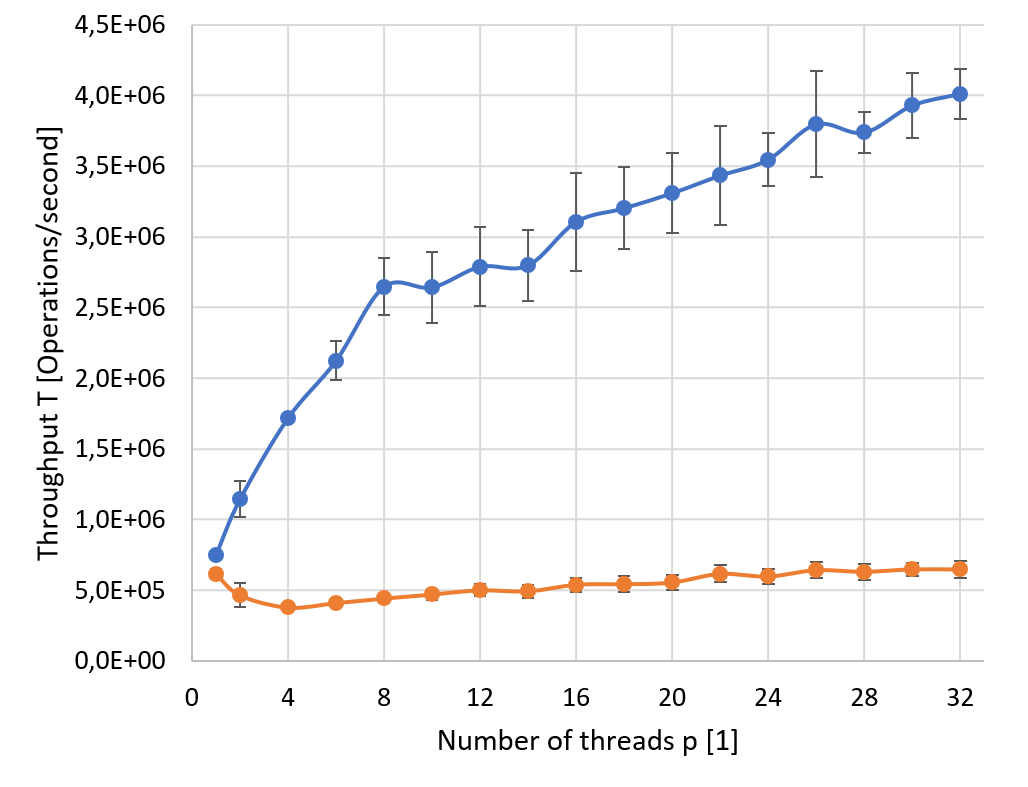
\includegraphics[width=9cm]{tp_vs_p.png}
\centering
\caption{Throughput of the wait-free (orange) and the lock-free (blue) list in the first benchmark with $i = 1\mathrm{E}6$ operations}
\label{tp_p}
\end{figure}

Figure \ref{tp_p} shows the result of the first benchmark. It is evident that the wait-free list performs significantly worse than its lock-free equivalent. For $p=1$ the performance is similar, the wait-free implementation is slightly slower because of its overhead. However, with  an increasing number of threads, the lock-free list scales well until $p=8$ (it reaches a speed-up of $3.5$ for 8 threads and $5.33$ for 32 threads) while the lock-free list does hardly gain any throughput from additional threads (speed-up of $1.05$ for 32 threads). Very similar behaviour was observed by the authors of \cite{timnat12}. The reason for the inferior performance of the wait-free list is the circumstance, that due to the helper scheme all threads try to execute one single operation until it is completed. This problem can be overcome partially by optimisations as shown in \cite{timnat12}.

Lists are generally not very efficient data structures as many operations have to iterate over all elements, yielding a complexity of $\mathcal{O}(n)$ for search operations. This causes problems for concurrent data structures. In case one CAS operation fails, it might be necessary to reiterate over the whole list. In order to study this effect, some CAS failures were counted during the benchmark. In order to meaningfully compare the wait-free and the lock-free list, failures of the following three CAS operations (which occur in both implementations) were counted\footnote{The wait-free list has several additional CAS operations, primarily modifying to the state array. These were not counted as they mostly do not require a list reiteration in case of failure}.
\begin{itemize}
\setlength\itemsep{0em}
\item{$CAS_{ADD}$: updates the \verb|next| pointer of the element in the list after which a new element is inserted (linking in)}
\item{$CAS_{REM, logical}$: updates the \verb|next| pointer of an element to be removed by setting the marked flag (logical deletion)}
\item{$CAS_{REM, physical}$: updates the \verb|next| pointer of the predecessor of an element to be removed (linking out, physical deletion)}
\end{itemize}

\begin{figure} [h!]
\begin{subfigure}[c]{0.45\textwidth}
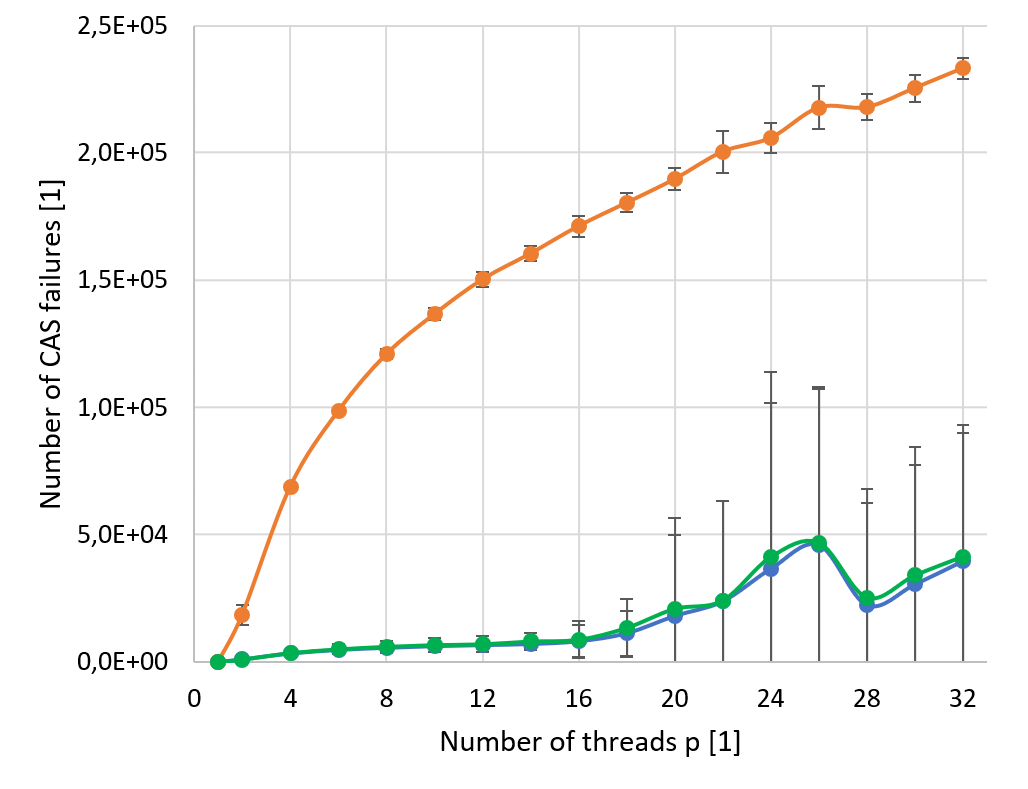
\includegraphics[width=7.5cm]{cas_vs_p_wf.png}
\centering
\end{subfigure}
\begin{subfigure}[c]{0.45\textwidth}
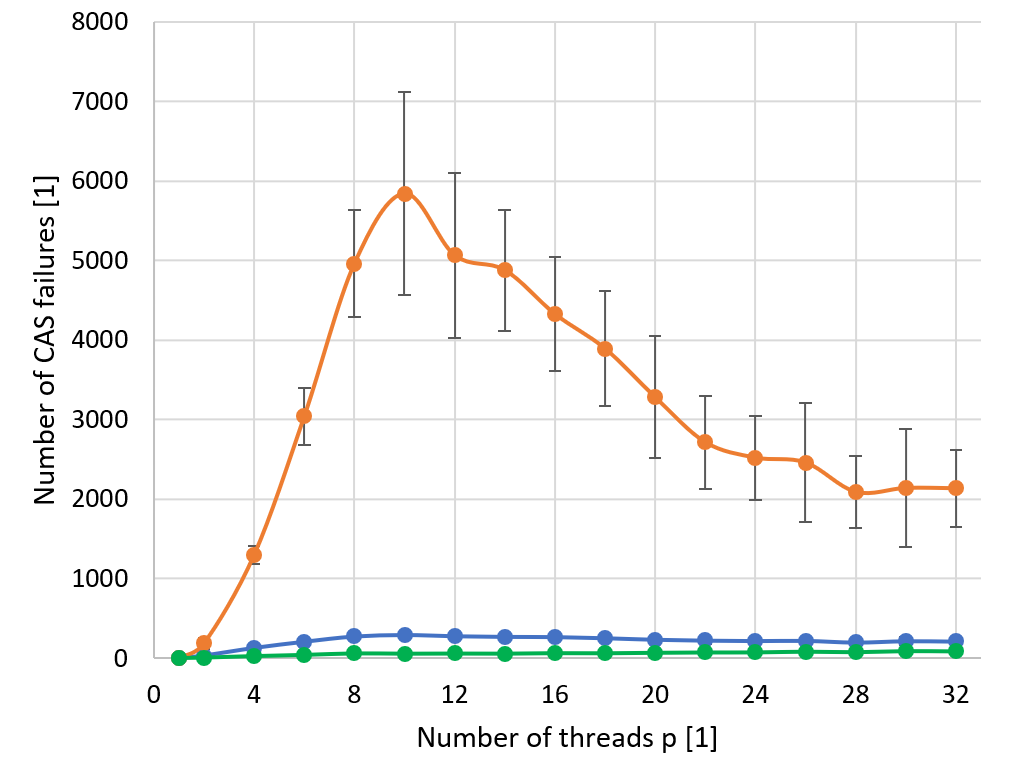
\includegraphics[width=7.5cm]{cas_vs_p_lf.png}
\centering
\end{subfigure}
\caption{Number of CAS failures for the wait-free (left) and the lock-free (right) list in the first benchmark with $i = 1\mathrm{E}6$ operations. The orange curve depicts the $CAS_{REM, physical}$ failures, the green curve the $CAS_{REM, logical}$ failures and the blue curve the $CAS_{ADD}$ failures.}
\label{cas_p}
\end{figure}

The number of CAS failures is a good indicator for the contention of a concurrent list. Figure \ref{cas_p} compares the number of CAS failures for the wait-free and the lock-free list during the first benchmark. Two findings can be derived from these results:
\begin{enumerate}
\item{The $CAS_{REM, physical}$ failures dominate over the other CAS failures in both cases. This might be due to the fact that the physical removal happens in the \verb|find| method, which is called by the \verb|add| as well as by the \verb|remove| method in both implementations.}
\item{The fact that all threads in the wait-free list try to help pending operations before execution their own request causes massive contention. As several threads are doing this simultaneously and only one of them can eventually succeed, the number of CAS failures is not only significantly higher than for the lock-free list but also increases with the number of threads. The fact that a CAS failure forces the thread to return to the beginning of the list explains why the performance of the wait-free implementation is far below the performance of the lock-free counterpart. Furthermore it is apparent that reduced helping (as proposed in \cite{timnat12}) can alleviate this problem.}
\end{enumerate}

So far the performance of the concurrent lists was examined as a function of the number of threads. Another interesting aspect is how well the data structures scale with the number of operations on the list. The results of the previous benchmark as a function of the number of random operations is depicted in Figure \ref{performance_i}.

\begin{figure} [h!]
\begin{subfigure}[c]{0.45\textwidth}
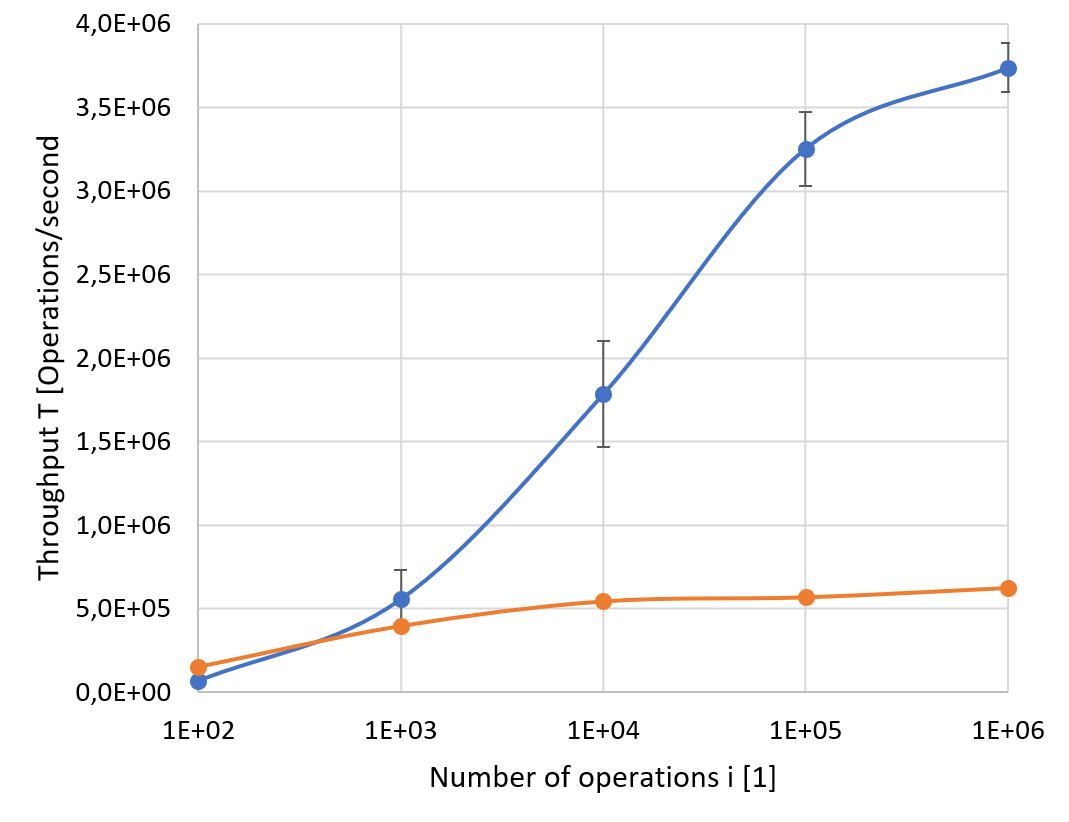
\includegraphics[width=7.5cm]{tp_vs_i.png}
\centering
\subcaption{Throughput}
\end{subfigure}
\begin{subfigure}[c]{0.45\textwidth}
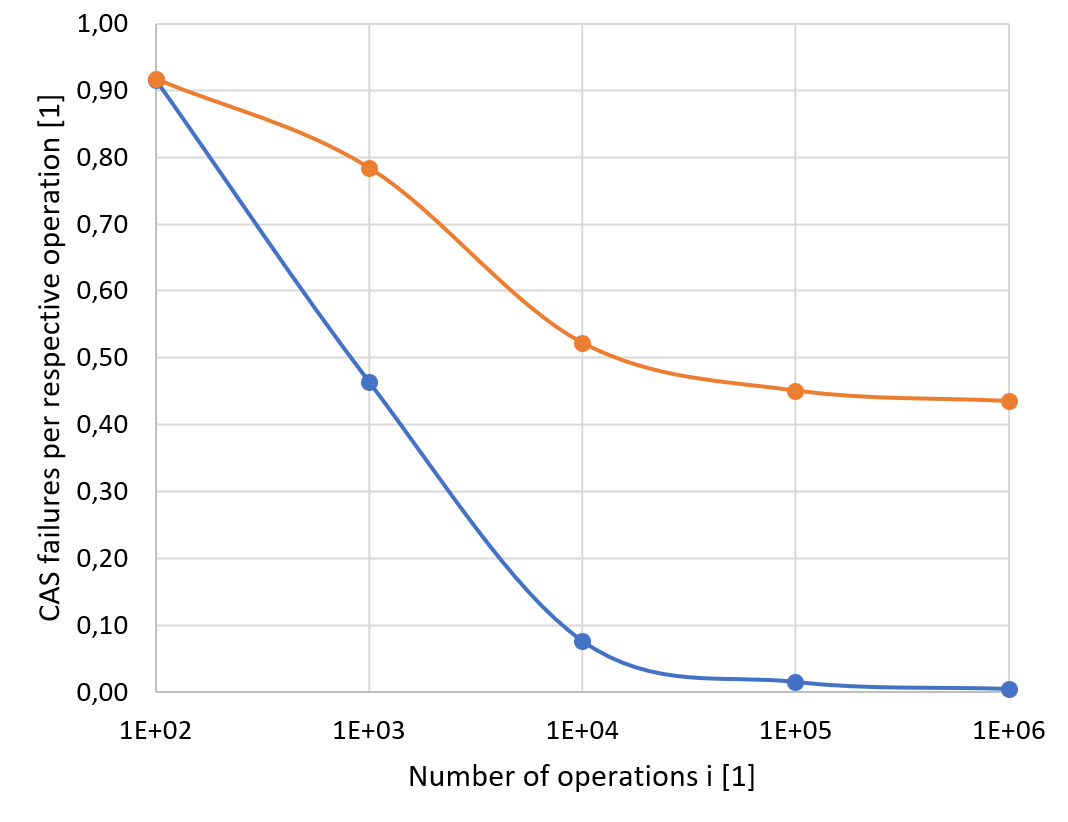
\includegraphics[width=7.5cm]{cas_rem_vs_i.png}
\centering
\subcaption{Number of $CAS_{REM, physical}$ failures per remove operation.}
\end{subfigure}
\caption{Performance measures of the wait-free (orange) and the lock-free (blue) list as function of the number of random operations in the first benchmark with 28 threads.}
\label{performance_i}
\end{figure}

Again, there are notable differences between the two list implementations. The throughput of the lock-free list increases with the number of operations while the wait-free list hardly scales with the problem size. The reason for this behaviour can be found in the number of $CAS_{REM, physical}$ failures. Both lists show massive contention as long as the number of operations is in the same magnitude as the number of threads. For a larger problem size the only a few per cent of the lock-free remove operations result in a $CAS_{REM, physical}$ failure, while the $CAS_{REM, physical}$ failure rate remains around $45\,\%$ for the wait-free list. This heavy contention explains the low throughput. It is worth noting here that the failure rates of the other CAS operations are in the low per cent range for both lists, so their influence on the performance is small compared to the logical deletion.

\subsection{Fill and clean-up phase}
In the first benchmark the list was filled with a constant number of items and random \verb|add| and \verb|remove| operations were executed in order to simulate a typical list operation. Another interesting aspect is the performance of the wait-free list in the fill and in the clean-up phase. So the \verb|add| and the \verb|remove| operation were studied in isolation. Again, integer values are used. It is important to mention that the \verb|add| and \verb|remove| operations in this benchmark do not add/remove random values. Each thread adds or removes $n/p$ sequential elements in increasing order ($n$ is the number of elements , $p$ the number of threads).

\begin{figure} [h!]
\begin{subfigure}[c]{0.45\textwidth}
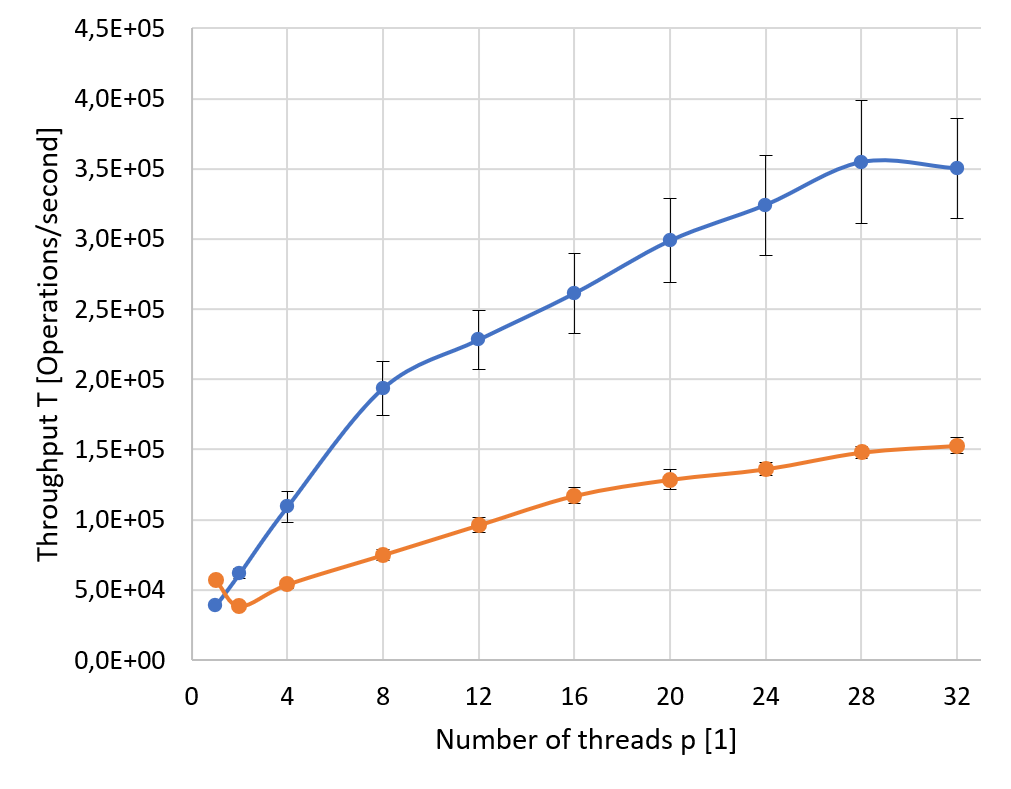
\includegraphics[width=7.5cm]{tp_fill.png}
\centering
\subcaption{Fill phase}
\end{subfigure}
\begin{subfigure}[c]{0.45\textwidth}
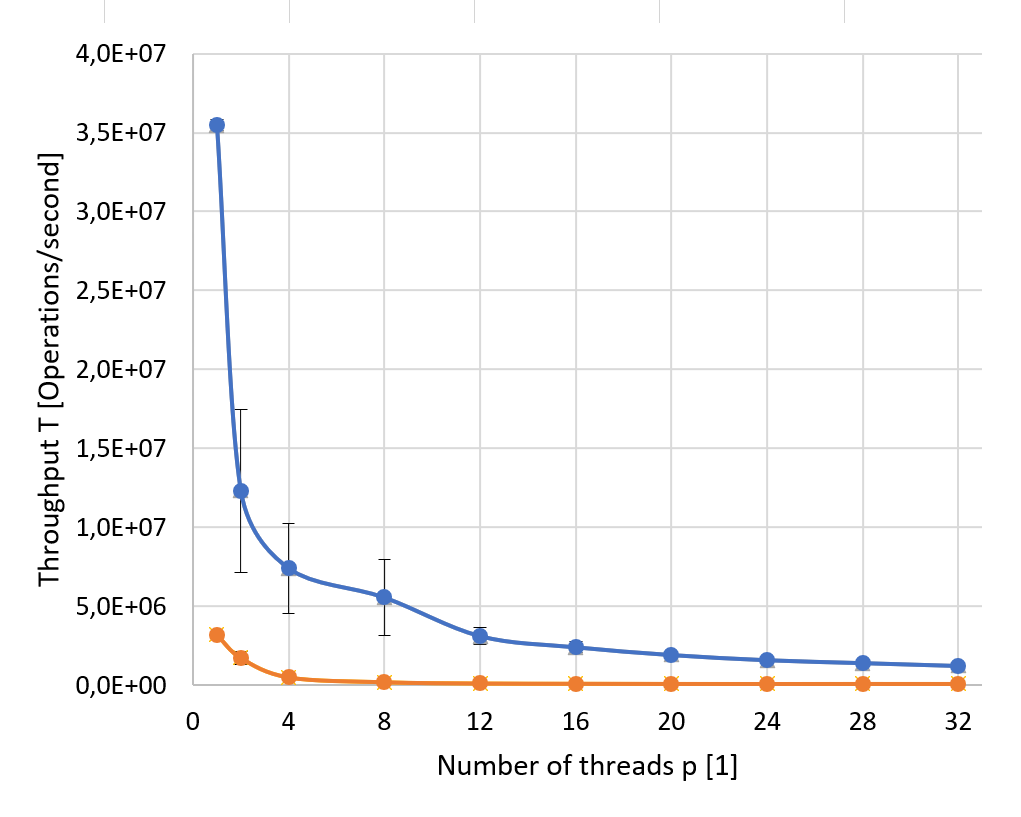
\includegraphics[width=7.5cm]{tp_cleanup.png}
\centering
\subcaption{Clean-up phase}
\end{subfigure}
\caption{Throughput of the wait-free (orange) and the lock-free (blue) list in the fill and the clean-up phase with $1E5$ elements.}
\label{tp}
\end{figure}

The main results of this benchmark are shown in Figure \ref{tp}. Two observations are particularly interesting: Firstly, the throughput of \verb|add| operations increases with the number of threads, while the \verb|remove| throughput decreases for both list implementations. Again, the frequency of CAS failures might explain this behaviour. While the $CAS_{ADD}$ and $CAS_{REM, logical}$ operations hardly fail, the $CAS_{REM, physical}$ miss rate increases with the number of threads and reaches up to $25\,\%$. Interestingly, there is hardly any difference between the wait-free and the lock-free list when it comes to CAS failures. As the $CAS_{REM, physical}$ operation is executed in the \verb|search| operation, which is called by every thread removing an item, collisions emerge and the \verb|remove| performance degrades with the number of threads. This does not happen with the \verb|add| method, as the addition of an element is finished once the method returns; there is no interdependence with other threads.

The second observation is that the performance of the wait-free list seems to be mainly limited by \verb|remove| operations. While the throughput of \verb|add| operations (in Figure \ref{tp}a) scales at least notably with the number of threads, this is not the case for the mix of operations assumed for the operational phase (which contains $50\,\%$ \verb|remove| operations, see Figure \ref{tp_p}). Even though the \verb|remove| throughput of the lock-free list is declining with the number of threads as well, the absolute numbers are still significantly higher than the \verb|add| throughput (e.g. $2.56E6$ Op/s for \verb|remove| and $1.58E5$ Op/s for \verb|add| with 32 threads in the benchmark depicted in Figure \ref{tp}). So in contrast to the wait-free list, the performance of the lock-free list is rather limited by the \verb|add| performance.

\section{Summary and Outlook}

The benchmarks showed that the performance of the basic wait-free list is significantly worse than the basic lock-free list used as reference in all tested configurations. To exploit the favourable progress guarantees, optimisations like the ones proposed in \cite{timnat12} are necessary. Whether these improvements ensure a reasonable performance for a wide variety of environment parameters has to be obtained by further benchmarking.

Another open issue is whether the wait-free list is a practically relevant data structure at all. Even though lists allow multiple concurrent read, add, and remove operations, the penalty for reiteration in case of a CAS failure is high and sequential data structure analysis shows that lists are no well-optimised data structures for many purposes.

\pagebreak
\sloppy
\printbibliography

\end{document}